% Created by tikzDevice version 0.12 on 2019-02-01 12:07:11
% !TEX encoding = UTF-8 Unicode
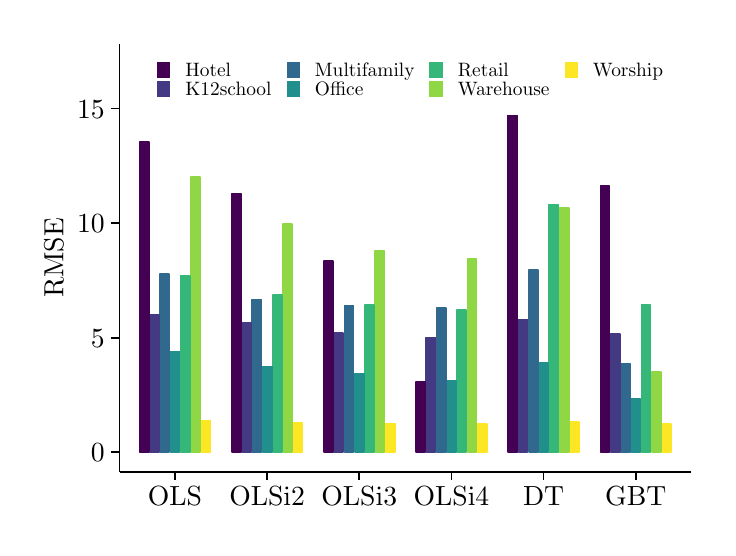
\begin{tikzpicture}[x=1pt,y=1pt]
\definecolor{fillColor}{RGB}{255,255,255}
\path[use as bounding box,fill=fillColor,fill opacity=0.00] (0,0) rectangle (245.72,180.67);
\begin{scope}
\path[clip] (  0.00,  0.00) rectangle (245.72,180.67);
\definecolor{drawColor}{RGB}{255,255,255}
\definecolor{fillColor}{RGB}{255,255,255}

\path[draw=drawColor,line width= 0.6pt,line join=round,line cap=round,fill=fillColor] (  0.00,  0.00) rectangle (245.72,180.68);
\end{scope}
\begin{scope}
\path[clip] ( 33.23, 20.23) rectangle (239.72,174.67);
\definecolor{fillColor}{RGB}{255,255,255}

\path[fill=fillColor] ( 33.23, 20.23) rectangle (239.72,174.67);
\definecolor{drawColor}{RGB}{253,231,37}
\definecolor{fillColor}{RGB}{253,231,37}

\path[draw=drawColor,line width= 0.6pt,line join=round,fill=fillColor] ( 62.68, 27.25) rectangle ( 66.01, 38.76);
\definecolor{drawColor}{RGB}{143,215,68}
\definecolor{fillColor}{RGB}{143,215,68}

\path[draw=drawColor,line width= 0.6pt,line join=round,fill=fillColor] ( 58.97, 27.25) rectangle ( 62.30,126.59);
\definecolor{drawColor}{RGB}{53,183,121}
\definecolor{fillColor}{RGB}{53,183,121}

\path[draw=drawColor,line width= 0.6pt,line join=round,fill=fillColor] ( 55.26, 27.25) rectangle ( 58.59, 91.00);
\definecolor{drawColor}{RGB}{33,144,140}
\definecolor{fillColor}{RGB}{33,144,140}

\path[draw=drawColor,line width= 0.6pt,line join=round,fill=fillColor] ( 51.55, 27.25) rectangle ( 54.88, 63.68);
\definecolor{drawColor}{RGB}{49,104,142}
\definecolor{fillColor}{RGB}{49,104,142}

\path[draw=drawColor,line width= 0.6pt,line join=round,fill=fillColor] ( 47.84, 27.25) rectangle ( 51.17, 91.74);
\definecolor{drawColor}{RGB}{68,58,131}
\definecolor{fillColor}{RGB}{68,58,131}

\path[draw=drawColor,line width= 0.6pt,line join=round,fill=fillColor] ( 44.12, 27.25) rectangle ( 47.45, 76.92);
\definecolor{drawColor}{RGB}{68,1,84}
\definecolor{fillColor}{RGB}{68,1,84}

\path[draw=drawColor,line width= 0.6pt,line join=round,fill=fillColor] ( 40.41, 27.25) rectangle ( 43.74,139.43);
\definecolor{drawColor}{RGB}{253,231,37}
\definecolor{fillColor}{RGB}{253,231,37}

\path[draw=drawColor,line width= 0.6pt,line join=round,fill=fillColor] ( 95.98, 27.25) rectangle ( 99.31, 37.85);
\definecolor{drawColor}{RGB}{143,215,68}
\definecolor{fillColor}{RGB}{143,215,68}

\path[draw=drawColor,line width= 0.6pt,line join=round,fill=fillColor] ( 92.27, 27.25) rectangle ( 95.60,109.62);
\definecolor{drawColor}{RGB}{53,183,121}
\definecolor{fillColor}{RGB}{53,183,121}

\path[draw=drawColor,line width= 0.6pt,line join=round,fill=fillColor] ( 88.56, 27.25) rectangle ( 91.89, 84.04);
\definecolor{drawColor}{RGB}{33,144,140}
\definecolor{fillColor}{RGB}{33,144,140}

\path[draw=drawColor,line width= 0.6pt,line join=round,fill=fillColor] ( 84.85, 27.25) rectangle ( 88.18, 58.21);
\definecolor{drawColor}{RGB}{49,104,142}
\definecolor{fillColor}{RGB}{49,104,142}

\path[draw=drawColor,line width= 0.6pt,line join=round,fill=fillColor] ( 81.14, 27.25) rectangle ( 84.47, 82.47);
\definecolor{drawColor}{RGB}{68,58,131}
\definecolor{fillColor}{RGB}{68,58,131}

\path[draw=drawColor,line width= 0.6pt,line join=round,fill=fillColor] ( 77.43, 27.25) rectangle ( 80.76, 74.02);
\definecolor{drawColor}{RGB}{68,1,84}
\definecolor{fillColor}{RGB}{68,1,84}

\path[draw=drawColor,line width= 0.6pt,line join=round,fill=fillColor] ( 73.72, 27.25) rectangle ( 77.05,120.72);
\definecolor{drawColor}{RGB}{253,231,37}
\definecolor{fillColor}{RGB}{253,231,37}

\path[draw=drawColor,line width= 0.6pt,line join=round,fill=fillColor] (129.29, 27.25) rectangle (132.62, 37.60);
\definecolor{drawColor}{RGB}{143,215,68}
\definecolor{fillColor}{RGB}{143,215,68}

\path[draw=drawColor,line width= 0.6pt,line join=round,fill=fillColor] (125.58, 27.25) rectangle (128.91, 99.94);
\definecolor{drawColor}{RGB}{53,183,121}
\definecolor{fillColor}{RGB}{53,183,121}

\path[draw=drawColor,line width= 0.6pt,line join=round,fill=fillColor] (121.87, 27.25) rectangle (125.20, 80.56);
\definecolor{drawColor}{RGB}{33,144,140}
\definecolor{fillColor}{RGB}{33,144,140}

\path[draw=drawColor,line width= 0.6pt,line join=round,fill=fillColor] (118.16, 27.25) rectangle (121.49, 55.65);
\definecolor{drawColor}{RGB}{49,104,142}
\definecolor{fillColor}{RGB}{49,104,142}

\path[draw=drawColor,line width= 0.6pt,line join=round,fill=fillColor] (114.44, 27.25) rectangle (117.78, 80.32);
\definecolor{drawColor}{RGB}{68,58,131}
\definecolor{fillColor}{RGB}{68,58,131}

\path[draw=drawColor,line width= 0.6pt,line join=round,fill=fillColor] (110.73, 27.25) rectangle (114.06, 70.22);
\definecolor{drawColor}{RGB}{68,1,84}
\definecolor{fillColor}{RGB}{68,1,84}

\path[draw=drawColor,line width= 0.6pt,line join=round,fill=fillColor] (107.02, 27.25) rectangle (110.35, 96.38);
\definecolor{drawColor}{RGB}{253,231,37}
\definecolor{fillColor}{RGB}{253,231,37}

\path[draw=drawColor,line width= 0.6pt,line join=round,fill=fillColor] (162.59, 27.25) rectangle (165.92, 37.43);
\definecolor{drawColor}{RGB}{143,215,68}
\definecolor{fillColor}{RGB}{143,215,68}

\path[draw=drawColor,line width= 0.6pt,line join=round,fill=fillColor] (158.88, 27.25) rectangle (162.21, 97.04);
\definecolor{drawColor}{RGB}{53,183,121}
\definecolor{fillColor}{RGB}{53,183,121}

\path[draw=drawColor,line width= 0.6pt,line join=round,fill=fillColor] (155.17, 27.25) rectangle (158.50, 78.58);
\definecolor{drawColor}{RGB}{33,144,140}
\definecolor{fillColor}{RGB}{33,144,140}

\path[draw=drawColor,line width= 0.6pt,line join=round,fill=fillColor] (151.46, 27.25) rectangle (154.79, 52.91);
\definecolor{drawColor}{RGB}{49,104,142}
\definecolor{fillColor}{RGB}{49,104,142}

\path[draw=drawColor,line width= 0.6pt,line join=round,fill=fillColor] (147.75, 27.25) rectangle (151.08, 79.41);
\definecolor{drawColor}{RGB}{68,58,131}
\definecolor{fillColor}{RGB}{68,58,131}

\path[draw=drawColor,line width= 0.6pt,line join=round,fill=fillColor] (144.04, 27.25) rectangle (147.37, 68.73);
\definecolor{drawColor}{RGB}{68,1,84}
\definecolor{fillColor}{RGB}{68,1,84}

\path[draw=drawColor,line width= 0.6pt,line join=round,fill=fillColor] (140.33, 27.25) rectangle (143.66, 52.67);
\definecolor{drawColor}{RGB}{253,231,37}
\definecolor{fillColor}{RGB}{253,231,37}

\path[draw=drawColor,line width= 0.6pt,line join=round,fill=fillColor] (195.90, 27.25) rectangle (199.23, 38.26);
\definecolor{drawColor}{RGB}{143,215,68}
\definecolor{fillColor}{RGB}{143,215,68}

\path[draw=drawColor,line width= 0.6pt,line join=round,fill=fillColor] (192.19, 27.25) rectangle (195.52,115.50);
\definecolor{drawColor}{RGB}{53,183,121}
\definecolor{fillColor}{RGB}{53,183,121}

\path[draw=drawColor,line width= 0.6pt,line join=round,fill=fillColor] (188.48, 27.25) rectangle (191.81,116.82);
\definecolor{drawColor}{RGB}{33,144,140}
\definecolor{fillColor}{RGB}{33,144,140}

\path[draw=drawColor,line width= 0.6pt,line join=round,fill=fillColor] (184.77, 27.25) rectangle (188.10, 59.45);
\definecolor{drawColor}{RGB}{49,104,142}
\definecolor{fillColor}{RGB}{49,104,142}

\path[draw=drawColor,line width= 0.6pt,line join=round,fill=fillColor] (181.05, 27.25) rectangle (184.38, 93.15);
\definecolor{drawColor}{RGB}{68,58,131}
\definecolor{fillColor}{RGB}{68,58,131}

\path[draw=drawColor,line width= 0.6pt,line join=round,fill=fillColor] (177.34, 27.25) rectangle (180.67, 75.27);
\definecolor{drawColor}{RGB}{68,1,84}
\definecolor{fillColor}{RGB}{68,1,84}

\path[draw=drawColor,line width= 0.6pt,line join=round,fill=fillColor] (173.63, 27.25) rectangle (176.96,167.65);
\definecolor{drawColor}{RGB}{253,231,37}
\definecolor{fillColor}{RGB}{253,231,37}

\path[draw=drawColor,line width= 0.6pt,line join=round,fill=fillColor] (229.20, 27.25) rectangle (232.53, 37.35);
\definecolor{drawColor}{RGB}{143,215,68}
\definecolor{fillColor}{RGB}{143,215,68}

\path[draw=drawColor,line width= 0.6pt,line join=round,fill=fillColor] (225.49, 27.25) rectangle (228.82, 56.31);
\definecolor{drawColor}{RGB}{53,183,121}
\definecolor{fillColor}{RGB}{53,183,121}

\path[draw=drawColor,line width= 0.6pt,line join=round,fill=fillColor] (221.78, 27.25) rectangle (225.11, 80.56);
\definecolor{drawColor}{RGB}{33,144,140}
\definecolor{fillColor}{RGB}{33,144,140}

\path[draw=drawColor,line width= 0.6pt,line join=round,fill=fillColor] (218.07, 27.25) rectangle (221.40, 46.54);
\definecolor{drawColor}{RGB}{49,104,142}
\definecolor{fillColor}{RGB}{49,104,142}

\path[draw=drawColor,line width= 0.6pt,line join=round,fill=fillColor] (214.36, 27.25) rectangle (217.69, 59.29);
\definecolor{drawColor}{RGB}{68,58,131}
\definecolor{fillColor}{RGB}{68,58,131}

\path[draw=drawColor,line width= 0.6pt,line join=round,fill=fillColor] (210.65, 27.25) rectangle (213.98, 70.05);
\definecolor{drawColor}{RGB}{68,1,84}
\definecolor{fillColor}{RGB}{68,1,84}

\path[draw=drawColor,line width= 0.6pt,line join=round,fill=fillColor] (206.94, 27.25) rectangle (210.27,123.53);
\end{scope}
\begin{scope}
\path[clip] (  0.00,  0.00) rectangle (245.72,180.67);
\definecolor{drawColor}{RGB}{0,0,0}

\path[draw=drawColor,line width= 0.6pt,line join=round] ( 33.23, 20.23) --
	( 33.23,174.67);
\end{scope}
\begin{scope}
\path[clip] (  0.00,  0.00) rectangle (245.72,180.67);
\definecolor{drawColor}{RGB}{0,0,0}

\node[text=drawColor,anchor=base east,inner sep=0pt, outer sep=0pt, scale=  1.00] at ( 27.83, 23.81) {0};

\node[text=drawColor,anchor=base east,inner sep=0pt, outer sep=0pt, scale=  1.00] at ( 27.83, 65.20) {5};

\node[text=drawColor,anchor=base east,inner sep=0pt, outer sep=0pt, scale=  1.00] at ( 27.83,106.59) {10};

\node[text=drawColor,anchor=base east,inner sep=0pt, outer sep=0pt, scale=  1.00] at ( 27.83,147.99) {15};
\end{scope}
\begin{scope}
\path[clip] (  0.00,  0.00) rectangle (245.72,180.67);
\definecolor{drawColor}{RGB}{0,0,0}

\path[draw=drawColor,line width= 0.6pt,line join=round] ( 30.23, 27.25) --
	( 33.23, 27.25);

\path[draw=drawColor,line width= 0.6pt,line join=round] ( 30.23, 68.64) --
	( 33.23, 68.64);

\path[draw=drawColor,line width= 0.6pt,line join=round] ( 30.23,110.04) --
	( 33.23,110.04);

\path[draw=drawColor,line width= 0.6pt,line join=round] ( 30.23,151.43) --
	( 33.23,151.43);
\end{scope}
\begin{scope}
\path[clip] (  0.00,  0.00) rectangle (245.72,180.67);
\definecolor{drawColor}{RGB}{0,0,0}

\path[draw=drawColor,line width= 0.6pt,line join=round] ( 33.23, 20.23) --
	(239.72, 20.23);
\end{scope}
\begin{scope}
\path[clip] (  0.00,  0.00) rectangle (245.72,180.67);
\definecolor{drawColor}{RGB}{0,0,0}

\path[draw=drawColor,line width= 0.6pt,line join=round] ( 53.21, 17.23) --
	( 53.21, 20.23);

\path[draw=drawColor,line width= 0.6pt,line join=round] ( 86.52, 17.23) --
	( 86.52, 20.23);

\path[draw=drawColor,line width= 0.6pt,line join=round] (119.82, 17.23) --
	(119.82, 20.23);

\path[draw=drawColor,line width= 0.6pt,line join=round] (153.13, 17.23) --
	(153.13, 20.23);

\path[draw=drawColor,line width= 0.6pt,line join=round] (186.43, 17.23) --
	(186.43, 20.23);

\path[draw=drawColor,line width= 0.6pt,line join=round] (219.74, 17.23) --
	(219.74, 20.23);
\end{scope}
\begin{scope}
\path[clip] (  0.00,  0.00) rectangle (245.72,180.67);
\definecolor{drawColor}{RGB}{0,0,0}

\node[text=drawColor,anchor=base,inner sep=0pt, outer sep=0pt, scale=  1.00] at ( 53.21,  7.94) {OLS};

\node[text=drawColor,anchor=base,inner sep=0pt, outer sep=0pt, scale=  1.00] at ( 86.52,  7.94) {OLSi2};

\node[text=drawColor,anchor=base,inner sep=0pt, outer sep=0pt, scale=  1.00] at (119.82,  7.94) {OLSi3};

\node[text=drawColor,anchor=base,inner sep=0pt, outer sep=0pt, scale=  1.00] at (153.13,  7.94) {OLSi4};

\node[text=drawColor,anchor=base,inner sep=0pt, outer sep=0pt, scale=  1.00] at (186.43,  7.94) {DT};

\node[text=drawColor,anchor=base,inner sep=0pt, outer sep=0pt, scale=  1.00] at (219.74,  7.94) {GBT};
\end{scope}
\begin{scope}
\path[clip] (  0.00,  0.00) rectangle (245.72,180.67);
\definecolor{drawColor}{RGB}{0,0,0}

\node[text=drawColor,rotate= 90.00,anchor=base,inner sep=0pt, outer sep=0pt, scale=  1.00] at ( 12.89, 97.45) {RMSE};
\end{scope}
\begin{scope}
\path[clip] (  0.00,  0.00) rectangle (245.72,180.67);
\definecolor{fillColor}{RGB}{255,255,255}

\path[fill=fillColor] ( 35.29,149.15) rectangle (235.60,174.67);
\end{scope}
\begin{scope}
\path[clip] (  0.00,  0.00) rectangle (245.72,180.67);
\definecolor{drawColor}{RGB}{68,1,84}
\definecolor{fillColor}{RGB}{68,1,84}

\path[draw=drawColor,line width= 0.6pt,line cap=round,fill=fillColor] ( 47.00,162.62) rectangle ( 51.27,167.96);
\end{scope}
\begin{scope}
\path[clip] (  0.00,  0.00) rectangle (245.72,180.67);
\definecolor{drawColor}{RGB}{68,58,131}
\definecolor{fillColor}{RGB}{68,58,131}

\path[draw=drawColor,line width= 0.6pt,line cap=round,fill=fillColor] ( 47.00,155.86) rectangle ( 51.27,161.20);
\end{scope}
\begin{scope}
\path[clip] (  0.00,  0.00) rectangle (245.72,180.67);
\definecolor{drawColor}{RGB}{49,104,142}
\definecolor{fillColor}{RGB}{49,104,142}

\path[draw=drawColor,line width= 0.6pt,line cap=round,fill=fillColor] ( 93.84,162.62) rectangle ( 98.11,167.96);
\end{scope}
\begin{scope}
\path[clip] (  0.00,  0.00) rectangle (245.72,180.67);
\definecolor{drawColor}{RGB}{33,144,140}
\definecolor{fillColor}{RGB}{33,144,140}

\path[draw=drawColor,line width= 0.6pt,line cap=round,fill=fillColor] ( 93.84,155.86) rectangle ( 98.11,161.20);
\end{scope}
\begin{scope}
\path[clip] (  0.00,  0.00) rectangle (245.72,180.67);
\definecolor{drawColor}{RGB}{53,183,121}
\definecolor{fillColor}{RGB}{53,183,121}

\path[draw=drawColor,line width= 0.6pt,line cap=round,fill=fillColor] (145.49,162.62) rectangle (149.76,167.96);
\end{scope}
\begin{scope}
\path[clip] (  0.00,  0.00) rectangle (245.72,180.67);
\definecolor{drawColor}{RGB}{143,215,68}
\definecolor{fillColor}{RGB}{143,215,68}

\path[draw=drawColor,line width= 0.6pt,line cap=round,fill=fillColor] (145.49,155.86) rectangle (149.76,161.20);
\end{scope}
\begin{scope}
\path[clip] (  0.00,  0.00) rectangle (245.72,180.67);
\definecolor{drawColor}{RGB}{253,231,37}
\definecolor{fillColor}{RGB}{253,231,37}

\path[draw=drawColor,line width= 0.6pt,line cap=round,fill=fillColor] (194.29,162.62) rectangle (198.56,167.96);
\end{scope}
\begin{scope}
\path[clip] (  0.00,  0.00) rectangle (245.72,180.67);
\definecolor{drawColor}{RGB}{0,0,0}

\node[text=drawColor,anchor=base west,inner sep=0pt, outer sep=0pt, scale=  0.70] at ( 56.98,162.88) {Hotel};
\end{scope}
\begin{scope}
\path[clip] (  0.00,  0.00) rectangle (245.72,180.67);
\definecolor{drawColor}{RGB}{0,0,0}

\node[text=drawColor,anchor=base west,inner sep=0pt, outer sep=0pt, scale=  0.70] at ( 56.98,156.12) {K12school};
\end{scope}
\begin{scope}
\path[clip] (  0.00,  0.00) rectangle (245.72,180.67);
\definecolor{drawColor}{RGB}{0,0,0}

\node[text=drawColor,anchor=base west,inner sep=0pt, outer sep=0pt, scale=  0.70] at (103.82,162.88) {Multifamily};
\end{scope}
\begin{scope}
\path[clip] (  0.00,  0.00) rectangle (245.72,180.67);
\definecolor{drawColor}{RGB}{0,0,0}

\node[text=drawColor,anchor=base west,inner sep=0pt, outer sep=0pt, scale=  0.70] at (103.82,156.12) {Office};
\end{scope}
\begin{scope}
\path[clip] (  0.00,  0.00) rectangle (245.72,180.67);
\definecolor{drawColor}{RGB}{0,0,0}

\node[text=drawColor,anchor=base west,inner sep=0pt, outer sep=0pt, scale=  0.70] at (155.47,162.88) {Retail};
\end{scope}
\begin{scope}
\path[clip] (  0.00,  0.00) rectangle (245.72,180.67);
\definecolor{drawColor}{RGB}{0,0,0}

\node[text=drawColor,anchor=base west,inner sep=0pt, outer sep=0pt, scale=  0.70] at (155.47,156.12) {Warehouse};
\end{scope}
\begin{scope}
\path[clip] (  0.00,  0.00) rectangle (245.72,180.67);
\definecolor{drawColor}{RGB}{0,0,0}

\node[text=drawColor,anchor=base west,inner sep=0pt, outer sep=0pt, scale=  0.70] at (204.27,162.88) {Worship};
\end{scope}
\end{tikzpicture}
